\section{Auswertung}
\label{sec:Auswertung}
Die Auswertung hat den Vergleich mehrerer Algorithmen des maschinellen Lernens zum Ziel.
Dafür werden die zur Verfügung gestellten Daten erst mit Pandas~\cite{pandas} vorprozessiert und auf ihnen mittels mRMR~\cite{mrmre} eine Attributselektion durchgeführt.

\subsection{Vorprozessierung}
Die zur Verfügung gestellten Datensätze bestehen aus insgesamt $\num{40000}$ Ereignissen.
Eine Hälfte davon sind Neutrinos (Signal), die andere Myonen (Untergrund).
Von diesen Ereignissen werden zuerst Attribute entfernt, die nicht in beiden Datensätzen vorhanden sind; es bleiben 237 Attribute übrig.
Dann werden unphysikalische Attribute, wie die IDs der Ereignisse und Informationen, die nur in der Simulation vorhanden sind, entfernt; es bleiben 188 Attribute übrig.
Dann werden Attribute mit einem Anteil an NaN-Werten von über 20\% entfernt; es bleiben 169 Attribute übrig.
Basis dafür ist die NaN-Verteilung in Abbildung~\ref{nanverteilung}.
Sie zeigt, dass die meisten Attribute weniger als 20\% NaNs enthalten.
Die etwa 19 Attribute mit einem Anteil größer 90\% enthalten nicht genügend Informationen für die Separation.
Die NaNs in den restlichen Attributen werden durch die Zahl -5000 ersetzt.
Eigentlich könnten alle NaNs auch zuerst mit dieser Zahl ersetzt werden und das Ausfiltern der Attribute mit zu vielen NaNs der Attributselektion überlassen werden.
Sind zu viele NaNs vorhanden entspricht dies einem geringen Informationsgehalt des Attributs, was automatisch erkannt werden sollte.
Konstante Attribute wurden auch nicht explizit entfernt, da diese vom mRMR automatisch herausgefiltert werden.
\begin{figure}
  \centering
  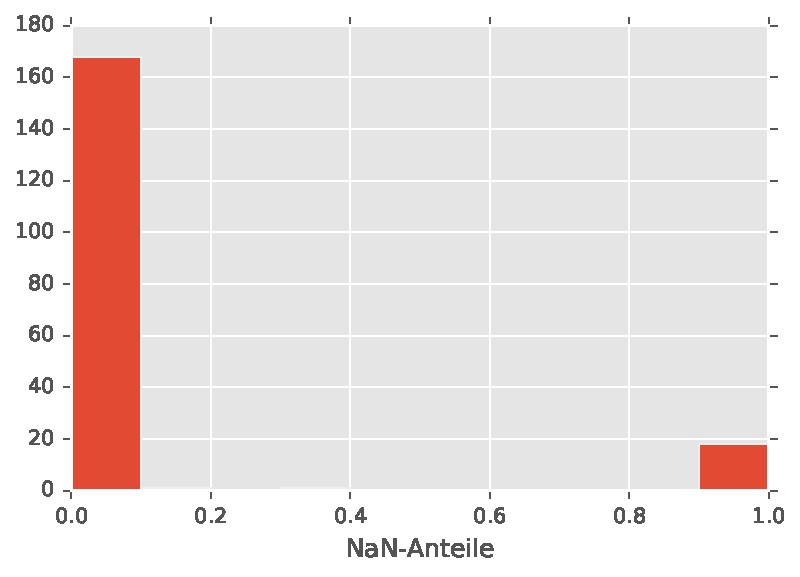
\includegraphics[width=0.80\textwidth]{nanplot}
\vspace{-1em}
  \caption{Histogramm der NaN-Anteile in den noch vorhandenen Attributen.}
  \label{nanverteilung}
\end{figure}


\subsection{Attributselektion}
Durchgeführt wird eine fünffache Attributselektion mittels mRMR.
Dafür werden aus der Menge der Gesamtereignisse fünf gleich große Ereigismengen mit zurücklegen gezogen und auf jeder dieser Mengen eine Attributselektion durchgeführt, um so eine Abschätzung der Varianz der Selektion zu erhalten. 
Die dafür verwendeten Ereignismengen wurden durch Ziehen mit Zurücklegen aus der Gesamtmenge von $\num{40000}$ Ereignissen erstellt.
Als Stabilität der Attributselektion wird der Jaccard-Index verwendet.
Die gemittelten Stabilitäten mit ihren Standardabweichungen gegen die Anzahl an selektierten Attributen $k$ sind in Abbildung~\ref{jaccardplot} zu sehen.
Die Mittelwerte steigen erst und sättigen sich bei $k=28$ zu etwa 0.9.
Hier ist auch die Standardabweichung der Mittelwerte am kleinsten.
Dieser $k$-Wert wird als Zahl der Attribute für die Separation gewählt.
Welche 28 Attribute genau ausgewählt werden, wird über eine eine Mehrheitsentscheidung der fünf Attributselektionen bestimmt.
Die 28 Attribute, die im Durchschnitt der Selektionen die höchsten Bewertungen erhalten, werden ausgewählt.
\begin{figure}
  \centering
  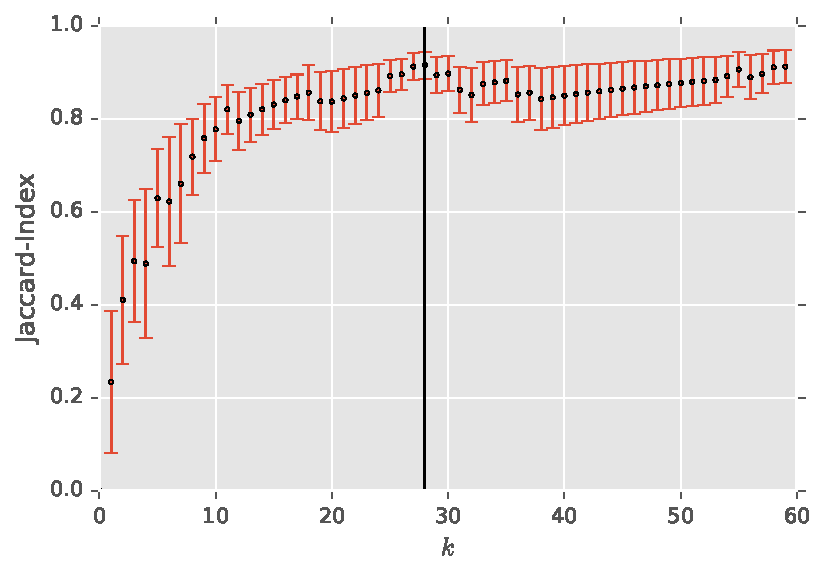
\includegraphics[width=0.80\textwidth]{jaccard}
\vspace{-1em}
  \caption{Die Mittelwerte der Jaccard-Indices mit ihren Standardabweichungen, gegen die Anzahl an selektierten Attributen.}
  \label{jaccardplot}
\end{figure}


\subsection{Separation}
Für die Separation werden innerhalb der Optimierung durch auto-sklearn~\cite{autosklearn} Algorithmen aus scikit-learn~\cite{scikit-learn} verwendet.
Außerdem wird noch der Naive-Bayes und Gradient Boosted Trees Operator aus RapidMiner~\cite{RapidMiner}, sowie der WEKA Random Forest~\cite{Weka2009} verwendet.


\subsubsection{Naive-Bayes}
Als Referenz für die Separationsqualitäten wurde der Naive-Bayes (NB) Algorithmus betrachtet.
Die gemittelten Reinheiten und Effizienzen aus der Kreuzvalidierung gegen die Konfidenz sind in Abbildung~\ref{naivebayes} zu finden.
Die Standardabweichungen des Mittelwerts sind als transparentes Band um die Mittelwerte eingezeichnet.
Der NB zeigt bereits eine sehr starke Trennung der beiden Klassen.
Die Reinheit steigt für größer werdende Konfidenzen nur in einem einstelligen Prozentbereich und erreicht einen maximalen Wert nahe 1.
Die Standardabweichungen sind im Verhältnis zu den Mittelwerten vernachlässigbar klein.
\begin{figure}
  \centering
  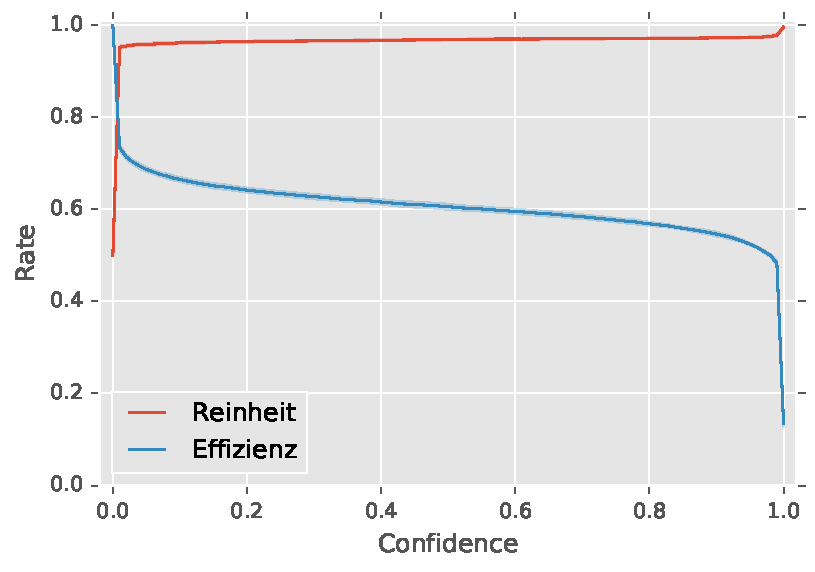
\includegraphics[width=0.80\textwidth]{bayesquality}
\vspace{-1em}
    \caption{Aufgetragen sind Mittelwerte der Reinheiten und Effizienzen mit ihren Standardabweichungen (als farbige Bänder) gegen die Konfidenz für den Naive-Bayes aus einer fünffachen Kreuzvalidierung.}
  \label{naivebayes}
\end{figure}

\subsubsection{Random Forest}
Der Random Forest wurde mit RapidMiner mit 200 Bäumen und dem Entropie Optimierungskriterium auf $\num{40000}$ Ereignissen trainiert.
Die Reinheit und Effizienz gegen die Konfidenz des Random Forests ist in Abbildung~\ref{figrndforestquality} dargestellt.
Der Random Forest zeigt ab Konfidenzen größer 0.5 eine höhere Reinheit als auch Effizienz als der NB.
Bei einer Konfidenz von 1.0 holt der NB in der Reinheit auf, während die Effizienz um etwa 25\% schlechter wird.
Die Standardabweichungen sind im Verhältnis zu den Mittelwerten vernachlässigbar klein.
\begin{figure}
  \centering
  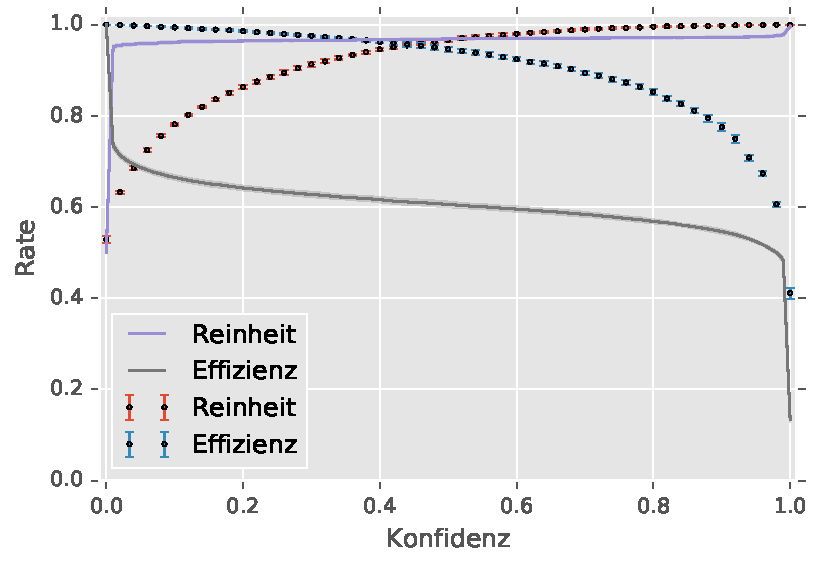
\includegraphics[width=0.80\textwidth]{rndforestquality}
\vspace{-1em}
    \caption{Aufgetragen sind Mittelwerte der Reinheit und Effizienz mit ihren Standardabweichungen gegen die Konfidenz für den Random Forest (Punkte) und den Naive-Bayes (durchzogene Linien) aus einer fünffachen Kreuzvalidierung. Die Standardabweichungen sind durch die farbigen Bänder und Fehlerbalken gekennzeichnet.}
  \label{figrndforestquality}
\end{figure}



\subsubsection{Gradient Boosting}
Die Algorithmenauswahl und Hyperparameterbestimmung erfolgt durch die Python Bibliothek auto-sklearn~\cite{autosklearn}, die ein Ensemble aus mehreren Lernern erstellt und ihre Hyperparameter anhand von selbst auswählbaren Qualitätskriterien optimiert.
Als zu maximierendes Kriterium wurde die der Anteil richtig Klassifizierter Ereignisse an der Gesamtmenge der Ereignisse gewählt.
Die zu verwendenden Algorithmen wurden über 27 Stunden optimiert.
Dabei hat auto-sklearn zuerst ein Gemisch aus Random Forests, Gradient Boosting und anderen Methoden verwendet.
Nach mehreren Stunden Rechenzeit wurden alle Algorithmen durch eine Kombination von 20 Gradient Boosting Lernern ersetzt.

Reinheit und Effizienz mit ihren Standardabweichungen gegen die Konfidenz sind in Abbildung~\ref{figaskquality} zu sehen.
Der Durchschnitt der Konfidenzen der einzelnen Lerner ist die Konfidenz des Ensembles.
Die Effizienz des auto-sklearn Ensembles ist für alle Konfidenzen außer 1.0 höher als die des Naive-Bayes.
Für Konfidenzen größer 0.5 zeigen sich, wie beim Random Forest, höhere Reinheiten als beim NB.
Die Standardabweichungen sind im Verhältnis zu den Mittelwerten vernachlässigbar klein.
\begin{figure}
  \centering
  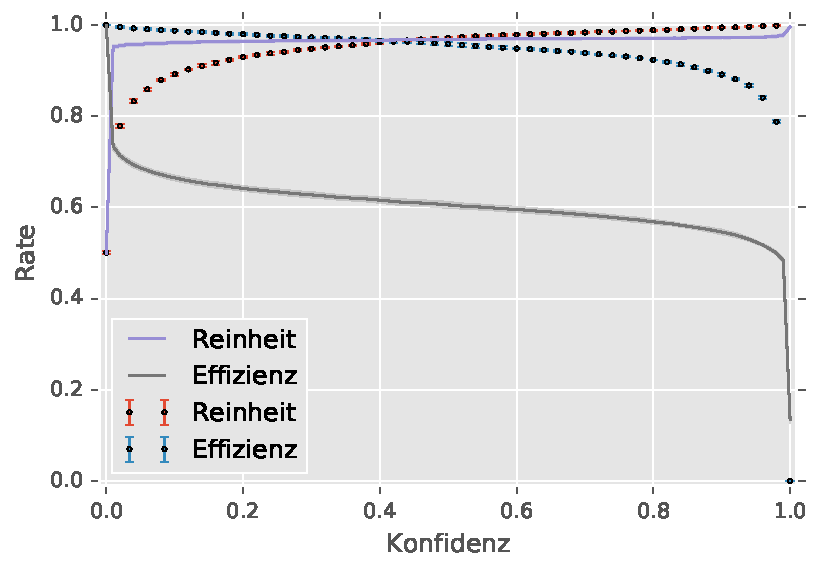
\includegraphics[width=0.80\textwidth]{askquality}
\vspace{-1em}
    \caption{Aufgetragen sind Mittelwerte der Reinheit und Effizienz mit ihren Standardabweichungen gegen die Konfidenz für das auto-sklearn ensemble (Punkte) und den Naive-Bayes (durchzogene Linien) aus einer fünffachen Kreuzvalidierung. Die Standardabweichungen sind durch die farbigen Bänder und Fehlerbalken gekennzeichnet.}
  \label{figaskquality}
\end{figure}

Abbildung~\ref{figrmgbquality} ist analog zu Abbildung~\ref{figaskquality} erstellt worden.
Es wurde hier das Gradient Boosting Ensemble von auto-sklearn durch den RapidMiner Gradient Boosted Trees Operator ersetzt.
Es zeigt sich ein sehr ähnliches Bild wie in Abbildung~\ref{figaskquality}.
\begin{figure}
  \centering
  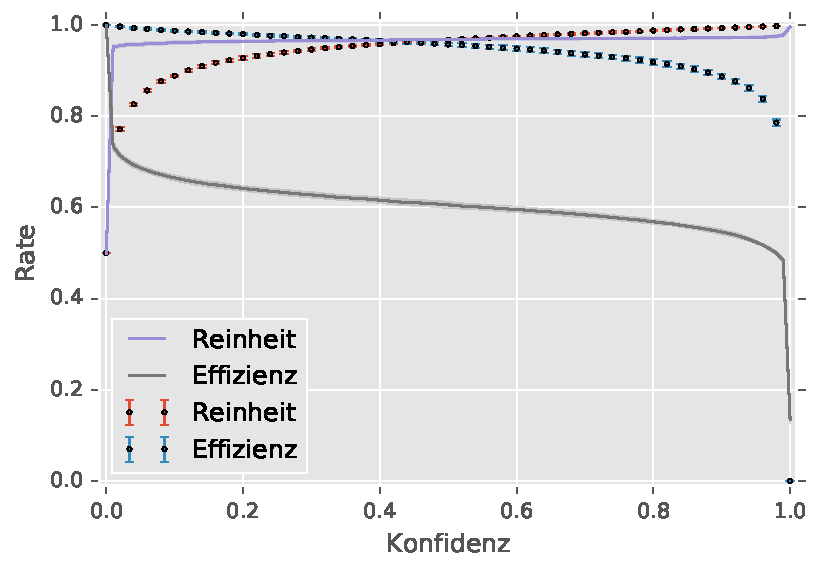
\includegraphics[width=0.80\textwidth]{rmgbquality}
\vspace{-1em}
    \caption{Aufgetragen sind Mittelwerte der Reinheit und Effizienz mit ihren Standardabweichungen gegen die Konfidenz für das den RapidMiner Gradient Boosted Trees Operator (Punkte) und den Naive-Bayes (durchzogene Linien) aus einer fünffachen Kreuzvalidierung. Die Standardabweichungen sind durch die farbigen Bänder und Fehlerbalken gekennzeichnet.}
  \label{figrmgbquality}
\end{figure}


\subsection{Vergleich der Gradient Boosted Trees}
Die Qualitätsunterschiede zwischen der RapidMiner Gradient Boosted Trees Implementierung und dem optimierten Ensemble von Gradient Boosted Trees aus auto-sklearn werden in Abbildung~\ref{figgbvsgb} in einem kleineren Ausschnitt verglichen.
Die durchzogenen Linien sind die Mittelwerte des auto-sklearn Ensembles.
Es zeigen sich nur geringe Abweichungen zwischen den beiden Lernern, die nur bei Konfidenzen um 0.5 größer als eine Standardabweichungen der beiden Lerner werden.
Die Lerner sind somit weitgehend äquivalent.
\begin{figure}
  \centering
  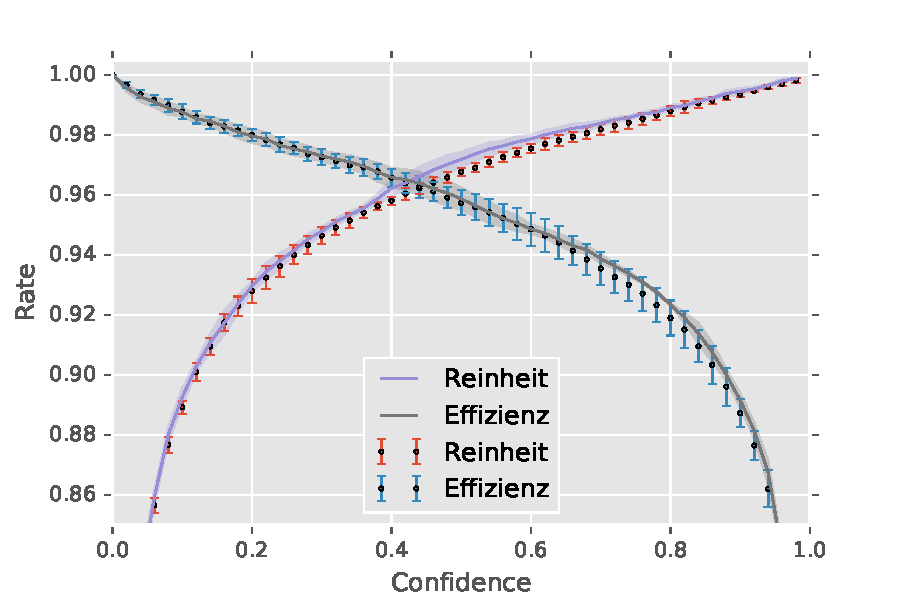
\includegraphics[width=0.80\textwidth]{gbvsgb}
\vspace{-1em}
    \caption{Aufgetragen sind Mittelwerte der Reinheit und Effizienz mit ihren Standardabweichungen gegen die Konfidenz für das auto-sklearn Ensemble (durchzogene Linien) und den RapidMiner Gradient Boosted Trees Operator (Punkte) aus einer fünffachen Kreuzvalidierung. Die Standardabweichungen sind durch die farbigen Bänder und Fehlerbalken gekennzeichnet.}
  \label{figgbvsgb}
\end{figure}


\subsection{Vergleich von Random Forest und Gradient Boosted Trees}
In Abbildung~\ref{figrfvsgb} wird der RapidMiner WEKA Random Forest Operator mit dem Gradient Boosted Trees (GBT) Operator verglichen.
Der GBT zeigt für alle Konfidenzen bis auf 1.0 eine höhere Effizienz, während für Konfidenzen größer 0.5 seine Reinheit leicht hinter der des Random Forests liegt.
Es ist zu beachten, dass für den GBT die Reinheiten für die selben Konfidenzen in diesem Bereich zwar niedriger als die des Random Forests sind, die Reinheiten des GBT für vorgegebene Werte der Effizienz aber höher als die des Random Forest sind.
Diese Überlegenheit des GBT gilt bis zu Reinheiten von 99.9\%, erst ab hier hat der GBT eine niedrigere Effizienz als der RF.
Die Effizienz des GBT wird dort gleich Null.
\begin{figure}
  \centering
  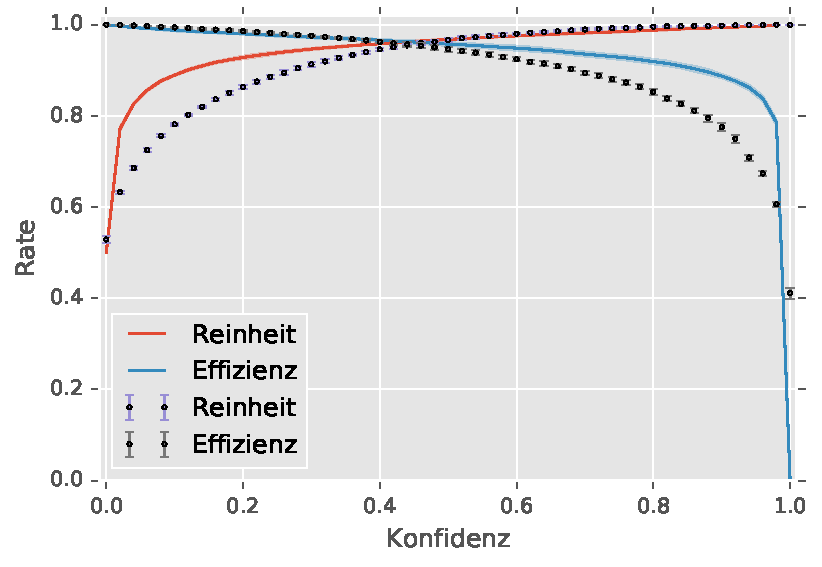
\includegraphics[width=0.80\textwidth]{rfvsgb}
\vspace{-1em}
    \caption{Aufgetragen sind Reinheit und Effizienz mit ihren Standardabweichungen gegen die Konfidenz für die RapidMiner Operatoren WEKA Random Forest (Punkte) und Gradient Boosted Trees (durchzogene Linien) aus einer fünffachen Kreuzvalidierung. Die Standardabweichungen sind durch die farbigen Bänder und Fehlerbalken gekennzeichnet.}
  \label{figrfvsgb}
\end{figure}






%oder einfach /input textable table
%\begin{table}
    %\sisetup{separate-uncertainty=true}
    %\centering
    %\caption{.}
    %\label{tab:1}
    %%\sisetup{table-format=2.1}
    %\begin{tabular}{l@{}S[table-format=-1.2, table-figures-uncertainty=1] S S S S}
        %\toprule
%%        & \multicolumn{2}{c}{Technetium} & \multicolumn{2}{c}{Molybdän} \\
        %%{} &
        %{\( /\si{} \)}  &  {\( /\si{} \)}  &  {\( /\si{} \)}  &  {\( /\si{} \)} \\
        %\midrule \input{messwerte/}
        %\bottomrule
    %\end{tabular}
%\end{table}
